\documentclass{llncs}

\usepackage{makeidx}
\usepackage{listings}
\usepackage{color}
%\usepackage{graphicx}
   \usepackage[pdftex]{graphicx}
   \usepackage[pdftex]{graphics}
\usepackage{float}
\usepackage{amsmath}
\usepackage{subfig}
\usepackage{cite}
\usepackage{url}
\usepackage{amsmath}
\usepackage[utf8]{inputenc}

\begin{document}


\title{Efficient dynamic and static environment classification in Occupancy Grid framework}
\author{
Jander Nascimento\inst{1,2}, \email{jander.botelho-do-nascimento@inria.fr} \and 
Qadeer Baig\inst{2}, \email{qadeer.baig@inria.fr} \and 
Mathias Perrollaz\inst{2}, \email{mathias.perrollaz@inria.fr}
}
\institute{
Université Joseph Fourier, 
621 av. Centrale - 38400 Saint-Martin-D'hères - FR
\and
Inria, \\
655 av. de l'Europe - Montbonnot - 38334 Saint Ismier Cedex - FR\\
}

\maketitle

\begin{abstract}

%replace fundamental by the word we use in the performance evaluation

Occupancy Grid are refereed in several literatures as an important tool to represent the surround environment of a robot, and working along with a statistical evaluation methods (e.g. importance sampling) is possible to perform clustering and classification of certain objects, Fast Clustering and Track Algorithms(FCTA). But in certain applications we do not have infinity processing power or enough samples. Thus, acquire certitude in the results takes longer and can compromise the \textit{killer application} of the algorithm, and the appearance of new objects that need to be tracked in the scene provoke steady space explosion, in which most of the times invalidates the real applicability of the solution. So we propose a method based in Bayesian Occupancy Filter that allows segmenting the static and dynamic environment with reduced number of frames, even though capable to distinguish these two environments with an acceptable accuracy, this possibility can be applied to other proposed solution to reduce the execution time for obtaining the results from output of the sensors. The algorithm was tested in a vehicle equipped with IBEO laser scanners.

\keywords{FCTA, Bayesian Occupancy Filter, Sensor fusion}

\end{abstract}

\section{Introduction}

In this document we are mainly concerned about driving assistance. However, driving assistance is a vast research field with almost a century of evolution. Such systems aims to support the driver in the action of driving, this support is given in any form: alerts, actuators to name few.

Since its appearance at the middle 50's, driving assistance has gained several branches, those branches have been heavily studied and contemporaneously are target of many research centers.

Drive-support systems are becoming more and more popular. The main reason for that is the increasing number of necessity to manage several instruments simultaneously into the vehicle\cite{riener2010sensor} and even follow up the action of the vehicles near by. The human non optimal, or even incapacity, of dealing with those situation engenders the need for drive-support systems.

Driving assistance engineering is not related to computer science. The first mechanisms ever created for driving assistance were related purely with mechanics, some examples of such systems are Cruise Control(CC), Anti Break System (ABS).

In this paper we concern mainly about driving assistance, thus, some issues faced by autonomous robotics are not in our scope, for instance: clustering, data association, tracking and mapping.

In vehicle time-line evolution, several techniques are concerned to improve the human ability and reaction when located behind a wheel, to name few: Anti-lock Break System(ABS), Adaptive Cruise Control(ACC), Collision Avoidance System(CAS).

For decades academics researchers have studying and trying to understand and mimic the human vision perception in the robotics field, as the vision is a ground bases for human condition, this has a trivial meaning through a human perspective, but mimic this characteristics is extremely complex.

Starting from vision, there exists several approaches and technologies that provide a representation of the environment: Radio frequency(RADAR), Electromagnet radiation (generally an invisible wave length), photograph representation. Those methods differentiate in the cost of equipment and the treatment in which their output must go through so the information can be used as an input.

The goal of having those representations, depending on the requirements of the application, is to track the objects, perform classification, data association, etc.

In this paper we are concerned with electromagnetic radiation scanners, LIDAR(Light Detection and Ranging) laser for instance.

The LIDAR laser scanners output is the basis for development of this work. As input of our algorithm we use Bayesian Occupancy Filter \cite{TAY-2008-295084} to cope with the uncertainty of the information given by the sensor measurements. As a rule of thumb the measurements require an estimation framework to correct, or least, approximate the measurements from the real data.

As our test platform is a vehicle, this kind of sensor is embedded in a vehicle as a set of sensors with different layers.

By the end of this report, we will present the results achieved and the uncertainty generated by the sensor measurements and its impacts in algorithm outputs.

\subsection{Spatial representation}

There exists several ways to represent one environment in with respect to its spatial information. Occupancy Grid is one of these methods and it is largely applied, its built based on a multidimensional field that maintains the occupancy state information in a cell\cite{Elfes:1989:UOG:68491.68495}. Those cells are built in a regular size, and the number of cells which compose the grid is algorithm dependent. 

At the same time Occupancy Grid (a.k.a. certainty grids) is effective in data representation it is also effective in represent sensor fusion information with it. Occupancy grid can be used as well to represent tree-dimentional environment, as was demonstrated in a small submersible craft, that looks for old battleships in the bottom of the ocean\cite{DBLP:journals/aim/Moravec88}.

One variation of the occupancy filter - The Bayesian Occupancy Filter(BOF) - contains the velocity and the probability distribution in Bayesian framework.


\subsubsection{SLAM}

SLAM (Simultaneous Localization and Mapping) is a concurrent map and localization problem, where the initial position of the ego-robot is unknown. The SLAM uses the observation done by the robot's sensor to localize the ego-robot in the environment and build the map at the same time\cite{VU-2009-454238}. 

But in this model it's required that we have a precise map - by precise we mean an exact map, exact enough for be considered as unreal and not achievable. This precision is required duo to simultaneously as the robot move we must localize it in the map, and as the robot motion is performed in a continuous space, any interference in the measurements are accumulated and can affect severely the localization.

The robot motion depends on the contact surface, inertial forces, the type of the ground surface in which the robot should move, its weight, speed, etc.

All those variations bring an imprecision factor into the movement performed by a robot.

From the probabilist point of view, this implies in estimate the joint probability distribution (Equation \ref{jpd:discrete}). Where the $u$ represents the observations and $z$ the measurements.

Thus, the output of the SLAM process is the robot pose and a map of the stationary objects captured by the \textit{perception} sensors \cite{iyengar1991autonomous}.

%\begin{equation}
%\label{jpd:continuous}
%\int_a^b f(x) \, \mathrm dx
%\end{equation}

\begin{equation}
\label{jpd:discrete}
P(x_t,M | z_{0:t}, u_{1:t})
\end{equation}


\subsubsection{DATMO}

Detection and Tracking of Moving Objects was initially studied by radar tracking systems \cite{VU-2009-454238} researches. Thus, they capture only moving object in the instrument, with those objects in scene they must solve the data association problem. The former assumption is unrealistic in the vision of a robot, the perception sensor senses all objects, independently on their motion, so static and dynamic objects are included.

As DATMO is a large process, some researchers chose to pick just a part of this process, which is "Moving Object Tracking" and solve it, without worry about the detection phase.

\subsubsection{SLAMMOT}

Researches considered SLAM and DATMO as two different problems that should be solved separately, \textit{Wang} was one of the first researches to put in evidence the similarities between both problems \cite{Wang03onlinesimultaneous}.

As result, the SLAMMOT term was coined and a derivation of the SLAM formula with DATMO was created to simplify the process of tracking. The experiment showed that solving the SLAM with DATMO increased dramatically the performance of the algorithm comparing them with the results as individual solutions (performance was verified in crowded urban environment).

As the GPS system or an good IMU for a good precision are too expensive, the paper propose a bayesian approach solution which satisties the navigation constraints without compromise the safety and at the sametime are not high costly as the other solutions based on a specialized hardware.

\subsubsection{SLAM and DATMO}

Robots face a set of problems which are common among many robots, how to move in a certain environment is one of them.

The general environment perception (Figure \ref{fig:perception:cycle}) requires at least two inputs: the perception measurements $Z$ which are usually are provided by cameras, LIDAR, or even radars, and motion measurements provided by the IMU (Inertial Measurement Unit).

\begin{figure}[H]
   \centering
     \begin{tabular}{lr}
       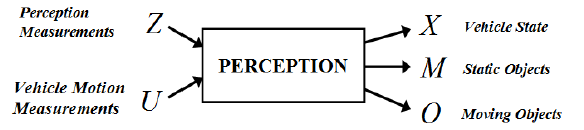
\includegraphics[scale=0.5]{img/fig:perception:cycle}
     \end{tabular}
   \caption{define}
   \label{fig:perception:cycle}
 \end{figure}


He perceives the environment by using as input sensors informations and can be composed of several sensors, or even heterogeneous types of sensors, and those give a partial observation of the environment (according with the current technology applied in those sensors). Thus, the robot does not known what paths can be perceived to reach a given point in a space.

So, knowing the positions that can be assumed by the robot is essential and necessary so robot cat move in this environment, this is done by observing the environment through the sensors and creating a spatial relation between the static objects in this space, this is known as SLAM - or Simultaneous Localizations and Mapping \cite{iyengar1991autonomous}.

Although, this just concern a small set of the problems related with robots applications, for instance robots that are used for mining, in this type of environment the only element that can change the environment and the spatial relation between the static objects is the robot itself. 

Depending in the goal of the robots perception, may be required to make distinction between each object, with cameras we can use characteristics like color, shape. Whereas, classify an object based in a LIDAR or radar information neither shape nor color are available, at least not directly without pre-processing.

Another set of problems concerns the most part of robots applications are highly dynamic environments, where the objects can change their position with respect to the static environment, those objects can become an obstacle for the robots, for this reason its necessary to map those objects, this relation called DATMO - Detection and Tracking of Moving Objects.

Although these two classification are given in a separate manner, they can be used as complementary to each other as presented in the paper \cite{Wang04a}, which will be dissected later.

\subsection{Occupancy grid mapping}

Representing continous space when dealing with the uncertainty of an action of a mobile robot is extremely demanding in terms of resource usage, either in terms of processing power or memory allocation.

Thus, targeting to amortize the computational requirement for the incertainty in the displacement of a robot, discretization models are used, Occupancy Grid\cite{Elfes:1989:UOG:68491.68495} is one of the former models proposed to tackle this issue.

This kind of representations is done with multi-dimensional vectors and results in a bird-eye view of the discretized map obtained by the perception sensor Figure \ref{fig:grid:continuous:discretized}.


\begin{figure}[H]
\centering
	\begin{tabular}{lr}\\
		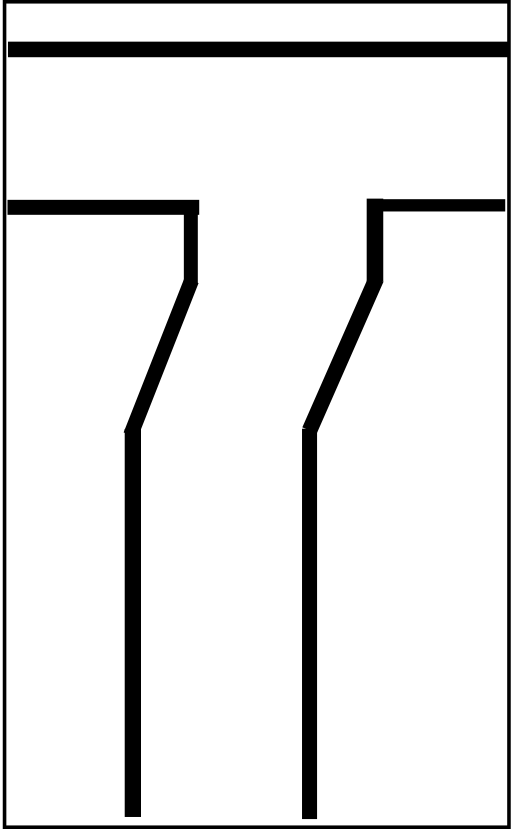
\includegraphics[width=0.25\columnwidth]{img/fig:grid:continuous} &
		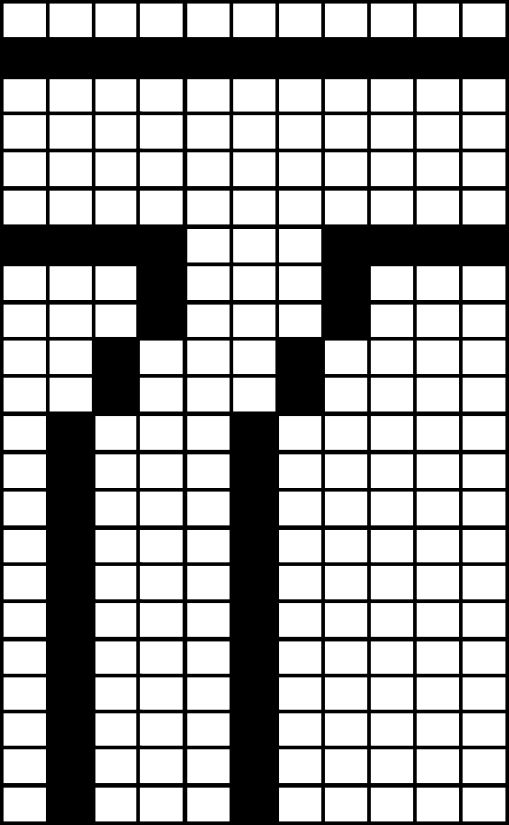
\includegraphics[width=0.25\columnwidth]{img/fig:grid:discretized}
	\end{tabular}
	\caption{Continuous \& discretized representation of a map}
	\label{fig:grid:continuous:discretized}
\end{figure}


In grid framework each cell $C$ can be assigned have its state $\phi(C)$ configured to binary domain, so, either the current state of the cell is \textit{occupied} or it is \textit{free}, in this paper we state that the value $1$ represents the occupied state and $0$ a $free$ space Equation \ref{eq:binarycell}.

\begin{equation}
P(\phi(C)=1) + P(\phi(C)=0) = 1
\label{eq:binarycell}
\end{equation}

This model can be extended to a more general model coined as \textit{inference grids} that encapsulate multiple properties\cite{Elfes:1989:OGP:916528}.

\textit{Goal: Why occupancy grid? how its built? }

\subsection{Object Separation}

\textit{Goal: u-disparity, uv-disparity}

\paragraph*{UV-disparity} 

UV disparity come off from an technique called U-disparity, a technique which aimed to separate the objects from the road surface.. (uv disparity slide 2)


\subsection{Classification}

\textit{Goal: talk about multimodels, importance sampling (or other statistical sampling method), prior map knowledge }

%multimodels, importance sampling, prior map knowledge

\section{State of the art}

\section{Experiment}

In the beginning of the experimentation phases, we modeled the algorithm to compute ahead of the time by using the bicycle model and extrapolating the pose by using the current vehicle measurements, like stearing angles. But this measurement had shown a lot of variation during a run, and the extrapolated model gets out to date very quickly.

From mechanical physics we obtain the angular velocity and from the vehicle \emph{CAN bus} we obtain the data time stamp, and along with it the time variation, $\Delta t$.

Using transformational matrices we bring the car perspective \cite{iyengar1991autonomous} and the prediction to the same frame of reference.

\section{Evaluation}

%target: dynamic and static separation, reduce the number of frames required, no classification, no association; no tracking, no 

\subsection{Testbed}

\subsubsection*{Hardware}

For testing purposes, we have a Lexus LS600h equipped with a stereo vision (TYZX camera) positioned in the superior part of the windshield.

The vehicle has two IBEO Lux Lidar in the front side of the car, one in each corner of the bumper.

As IMU, the car is equipped with a Xsens IMU and a GPS for global positioning.

As the test platform requires a powerfull computer to process the stereo images in realtime, the car is equipped with a Dell workstation with an NVidia graphic card.

DeepSea TYZX stereo vision camera has a base line of 22 cm with 512x320 pixels of resolution and focal length of 410 pixels, this camera is provided with a library which can estimate the distance in cm of the objects captured by the camera, but in our tests we used the estimators developed at Inria\cite{PERROLLAZ-2010-493397}.
%better references
%http://ieeexplore.ieee.org/stamp/stamp.jsp?tp=&arnumber=6170895
%http://hal.inria.fr/index.php?halsid=fa9c2loot97ptftt2n38f6lvr5&view_this_doc=hal-00671208&version=1

Each IBEO Lux Lidar is composed of four layers, each of them providing about 200 beams. The angular range of 100 degrees with angular resolution of 0.5 degrees. Each beam can reach until 200 m of distance measurement, with width of 40 m and maximum height of 2 m.

MTi-G XSens minimum of 120Hz and maximum of 512Hz for data logging and angular resolution of 0.05 degrees, all specifications are valid when considering an homogenous eletromagnetic environment. Maximum altitude operation is 18 Km and maximum speed is 515 m/s.

\begin{figure}[H]
   \centering
     \begin{tabular}{lr}
     \multicolumn{2}{c}{ 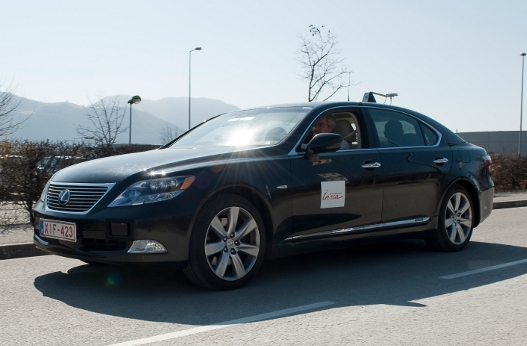
\includegraphics[width=0.55\columnwidth]{img/testbed:car}}\\
       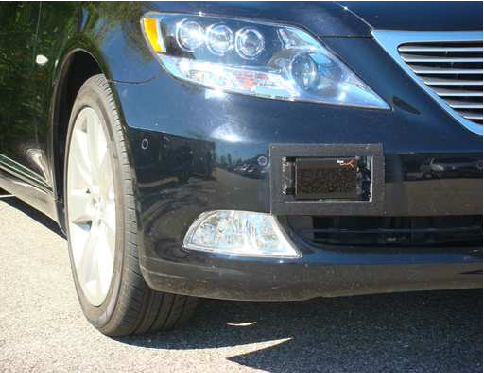
\includegraphics[width=0.42\columnwidth]{img/testbed:ibeo}
       &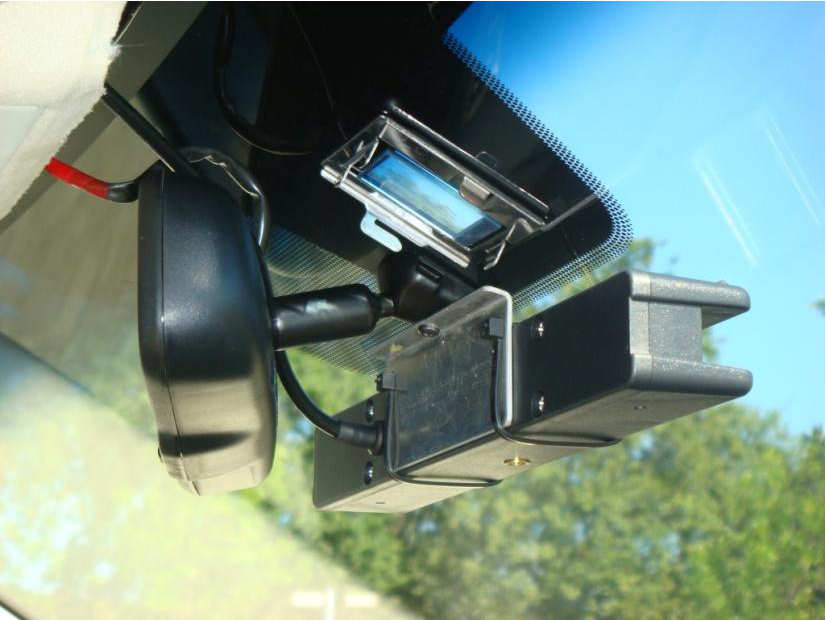
\includegraphics[width=0.42\columnwidth]{img/testbed:tyzx}
     \end{tabular}
   \caption{Lexus LS600h car equipped with two IBEO Lux lidars and a TYZX
     stereo camera}
   \label{fig:Lexus}
 \end{figure}

\begin{figure}[H]
   \centering
     \begin{tabular}{lr}
       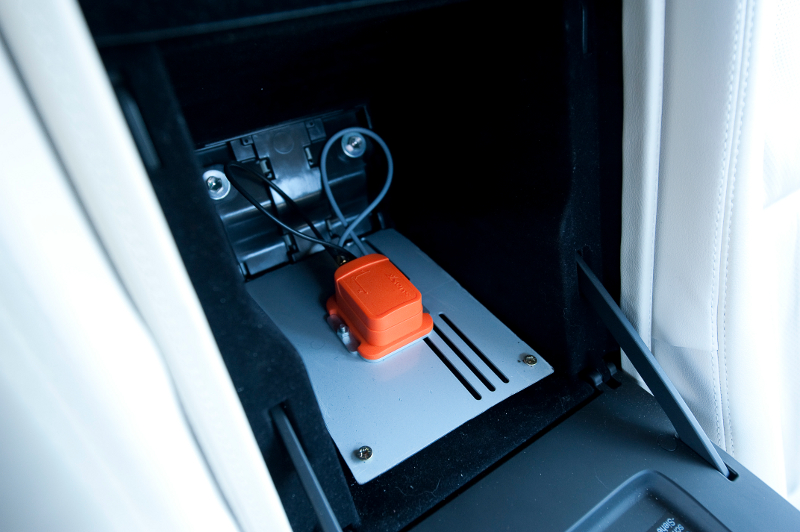
\includegraphics[width=0.55\columnwidth]{img/testbed:xsens}
       & 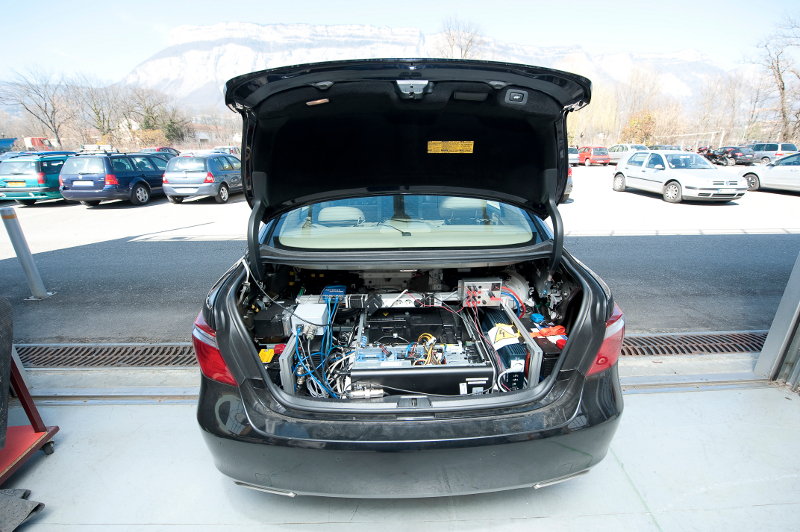
\includegraphics[width=0.55\columnwidth]{img/testbed:trunc}
     \end{tabular}
   \caption{MTi-G XSens IMU unit \& Intel Xeon 3.4GHz linux box}
   \label{fig:Lexus}
 \end{figure}


\subsubsection*{Software}

The high end cars are composed of several internal networks, each of them responsible to handle the transmission of the informations that are captured in that network to other one which need to process that information. This type of network is known as Controller Area Network (CAN) and provides a cheap and reliable way to communicate with devices, so CAN bus have been replacing the regular point-to-point wiring interconnection among the components\cite{bosch91can}.

Car manufacturers use platforms like YARP - Yet Another Robot Platform -, URBI or ROS to publish the information gathered by those networks, frameworks like ROS, allow the car to put the information into a shared memory array which can be access by other applications, the intent for most of those frameworks is to give longevity\cite{Fitzpatrick:2008:TLR:1327539.1327705} for the robot application that uses it by providing a platform that can evolve in cooperation manner with other projects.

For this project Robot Operating System(ROS) was adopted, ROS gives us the hability to save all information obtained during a run (driving the test platform) from all sensors, and replay it later in the laboratory, this by far allow to have a consistent test samples and a historical evolution of all scenarios gathered during the algorithm evolution, aloing the retro-performance benchmarking with other versions of the algorithm.

\subsubsection*{Assumptions}

\textit{Goal: What we assume to make our algorithm work}

\subsubsection*{Notation}

\paragraph{Occupancy Grid visual representation}

Representatiing the occupancy grid, implies in taking some precautions in the pattern used to represent each state, in this work the value $1$ represents occupied spaces and $0$ free spaces, although in the visual representation of the occupancy grid the $black$ dots represent occupied spaces and $white$ ones represent free spaces. In certain occasions, where the grid depicted is not binary, spaces where framework has absolutely no information about certain spaces (\textit{e.g.} due unreachability of the perception sensors in that sector), the color used is $gray$.

\subsection{Results}

\textit{Goal: What are our current results}

\subsection{Conclusion}

\textit{Goal: Express what we can conclude from this work, talk about future work, may be}

\bibliographystyle{plain}
\bibliography{report}{}

\end{document}



